\section{Vandermonde matrix}

For this exercise I needed to solve an equation containing a Vandermonde matrix using LU decomposition and Neville\'s algorithm.
Because I could copy all of the functions from the working classes, 
my code for those is similar to my sister\'s, Liz van der Kamp (s2135752). 
The only function not directly taken from my tutorial code is the one iterating on the LU solution to improve it, 
but the method for multiplying a matrix by a vector by doing np.sum(A*x, axis=1) I also took from my tutorial code in collaboration with Liz.

\subsection{a}
To read in the Vandermonde.txt file, I copied the example code provided in the Handin, 
then I generated the Vandermonde matrix and executed LU decomposition.
From the LU decomposition, I get the LU matrix, the solution for c, 
and an array of indexes which have saved which rowswaps I have done so I can reuse the LU matrix and my code later on without having to swap rows back.
Then, I get the interpolated result $y = \sum_j c_j x^j$ both for my 1000 x points and my initial x$_i$ so I can compare to the initial data points, 
and I plot the results in Fig. \ref{fig:fig1}.
The resulting solution for for c is:
\lstinputlisting{NUR1_c_sol1.txt}

\begin{figure}[h!]
  \centering
  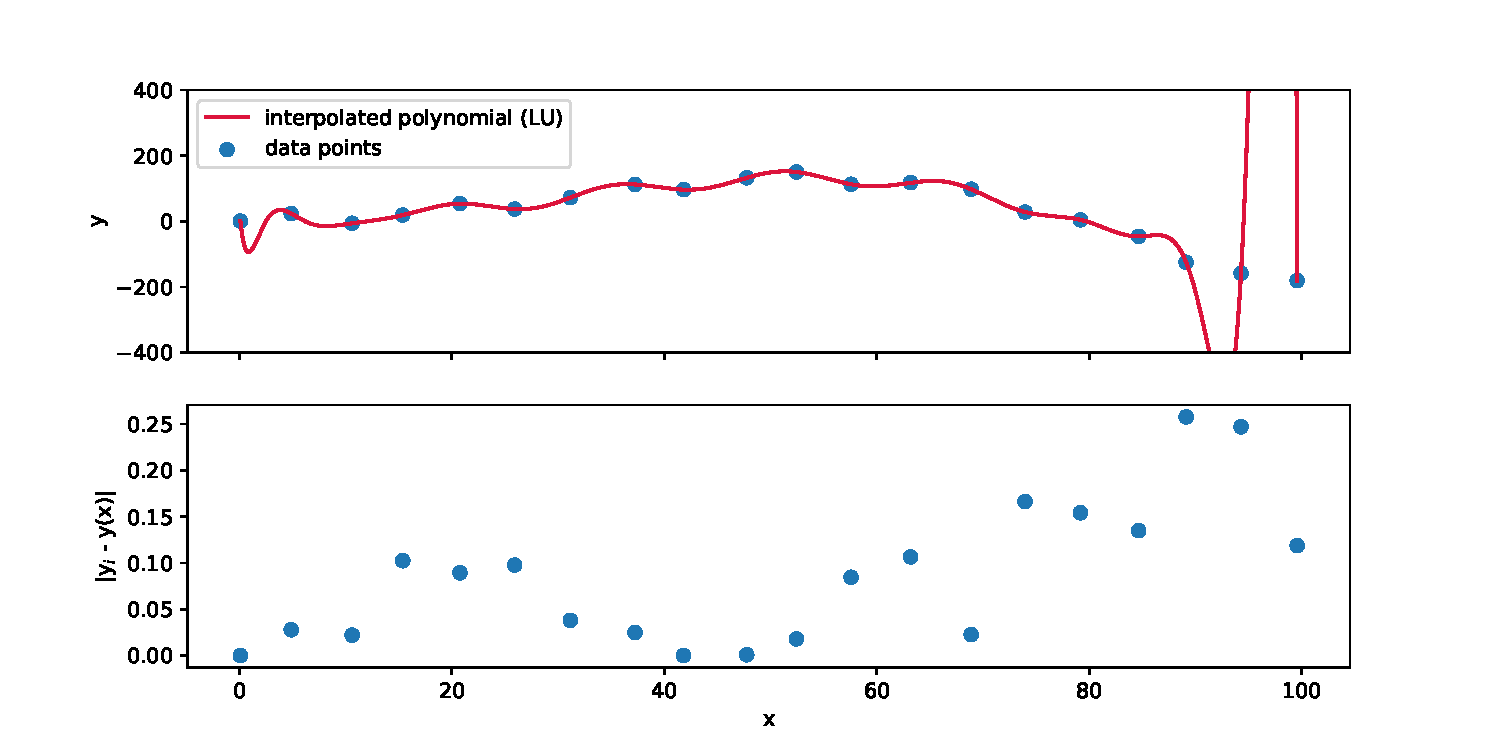
\includegraphics[width=0.9\linewidth]{./NUR1_Q2_plot1.pdf}
  \caption{Plot corresponding to exercise 2a. The top plot shows the data points 
  and the interpolated 19th degree polynomial given by the LU decomposition. The bottom plot shows the absolute difference between
  the data points and the result from the LU decomposition.}
  \label{fig:fig1}
\end{figure} 

\subsection{b}
